\documentclass[12pt,a4paper]{report}
\usepackage[english]{babel}
\usepackage[utf8x]{inputenc}
\usepackage{newlfont}
\usepackage{color}
\usepackage{hyperref}
\usepackage{amsmath}
\usepackage{graphicx}
\usepackage{epigraph}
\usepackage[overload]{empheq}
\usepackage[inline, shortlabels]{enumitem}
\usepackage{bm}

\usepackage{emptypage} % remove header in blanck pages

\usepackage[a4paper,top=4cm,bottom=4cm,left=3cm,right=3cm,marginparwidth=1.75cm]{geometry}

\hypersetup{
colorlinks,
citecolor=black,
filecolor=black,
linkcolor=black,
urlcolor=blue
}

\textwidth=450pt\oddsidemargin=0pt

\begin{document}
\begin{titlepage}
%
%
% ONCE YOU ARE FINISHED WITH YOUR CHANGES MODIFY "RED" WITH "BLACK" IN ALL \textcolor COMMENTS
%
%
\begin{center}
{{\Large{\textsc{Alma Mater Studiorum $\cdot$ University of  Bologna}}}} 
\rule[0.1cm]{15.8cm}{0.1mm}
\rule[0.5cm]{15.8cm}{0.6mm}
\\\vspace{3mm}
{\small{\bf School of Science \\
Department of Physics and Astronomy\\
Master Degree in Physics}}
\end{center}

\vspace{17mm}

\begin{center}
%
% INSERT THE TITLE OF YOUR THESIS
%
{\LARGE{\bf OPTIMIZATION AND APPLICATIONS\\
OF DEEP LEARNING ALGORITHMS\\
\vspace{3mm}
FOR SUPER-RESOLUTION IN MRI}}\\
\end{center}

\vspace{30mm} \par \noindent

\begin{minipage}[t]{0.47\textwidth}

{\large{\bf Supervisor: \vspace{2mm}\\
Prof. Gastone Castellani\\\\

\bf Co-supervisor:
\vspace{2mm}
\\
Dr. Nico Curti\\\\}}
\end{minipage}
%
\hfill
%
\begin{minipage}[t]{0.47\textwidth}\raggedleft \textcolor{black}{
{\large{\bf Submitted by:
\vspace{2mm}\\
Mattia Ceccarelli}}}
\end{minipage}

\vspace{40mm}

\begin{center}

Academic Year 2019/2020
\end{center}

\end{titlepage}

\newpage

\vspace*{125px}
\LARGE\textit{Abstract}
\normalsize
\vspace{2mm}

Abstract

\newpage
\normalsize 

\tableofcontents

\chapter{Introduction}

Brief introduction of the work

\section{Neural Network and Deep Learning}

A neural network is an interconnected structure of simple procedurals units, called nodes. Their functionality is inspired by the animals' brain and from the works on learning and neural plasticity of Donald Hebb \cite{hebb-learning}. From his book :

\begin{quote}
 \begin{center}
  \textit{Let us assume that the persistence or repetition of a reverberatory activity (or "trace") tends to induce lasting cellular changes that add to its stability.[…] When an axon of cell A is near enough to excite a cell B and repeatedly or persistently takes part in firing it, some growth process or metabolic change takes place in one or both cells such that A's efficiency, as one of the cells firing B, is increased}
 \end{center}
\end{quote}

which is an attempt to describe the change of strenght in neural relations as a consequence of stimulations.
From the so-called \textit{Hebbian Theory} rose the first computational models such as the \textit{Perceptron}, \textit{Neural Networks} and the modern \textit{Deep Learning}. 
The development of learning-based algorithms didn't catch up with the expected results until recently, mainly due to the exponential increase in available computational resources.

From a mathematical point of view, a neural network is a composition of non-linear multi-parametric functions. 
During the {\it training phase} the model tunes its parameters, starting from random ones, by minimizing the error function (called also loss or cost). 
Infact, machine learning problems are just optimization problems where the solution is not given in an analytical form, therefore trough iteratives techniques (generally some kind of gradient descent) we progressively approximate the correct result.

In general, there are 3 different kind of approach to learning:

\begin{itemize}
 \item {\bf supervised} It exists a labeled dataset in which the relationship between features (input) and expected output is known. 
 During training, the model is presented with many examples and it corrects its answers based on the correct response.  
 Some problems tied to supervised algorithms are classification, regression, object detection, segmentation and super-resolution.
 \item {\bf unsupervised} In this case, a labeled dataset does not exist, only the inputs data are available. 
 The training procedure must be tailored around the problem under study. Some examples of unsupervised algorithms are clustering, autoencoders, anomaly detection.
 \item {\bf reinforced} the model interacts with a dynamic environment and tries to reach a goal (e.g. winning in a competitive game). 
 For each iteration of the training process we assign a reward or a punishent, relatively to the progress in reaching the objective.
\end{itemize}

This work will focus on models trained using labeled samples, therefore in a supervised environment.

\subsection*{Perceptron}

The Perceptron (also called \textit{artificial neuron}) is the fundamental unit of every neural network and it is a simple model for a biological neuron, based on the works of Rosenblatt \cite{perceptron}. 
The \textit{perceptron} receives $N$ input values $x_1, x_2, ... x_N$ and the output is just a linear combination of the inputs plus a bias :

\begin{equation}
y = \sigma(\sum_{k=1}^N w_kx_k + w_0)
\end{equation}

where $\sigma$ is called \textit{activation function} and $w_0, w_1, ... w_N$ are the trainable weights.

Originally, the activation function was the \textit{Heaviside step function} whose value is zero for negative arguments and one for non-negative arguments: 

\begin{equation}
H(x) := 
\begin{cases}
  0 \text{ if } x < 0 \\ 
  1 \text{ if } x \geq 0 \\
\end{cases}
\end{equation}

In this case the perceptron is a \textit{linear discriminator} and as such, it is able to learn an hyperplane which linearly separates two set of data.
The weights are tuned during the training phase following the given update rule, usually :

\begin{equation}
 \bm{w}_{n+1} = \bm{w}_n + \eta (t - y)\bm{x}
 \label{eq:perceptron}
\end{equation}

where $\eta$ is the learning rate ($\eta \in [0,1]$) and $t$ is the true output. If the input instance is correctly classified,  the error $(t - y)$ would be zero and no weight is changed. 
Otherwise, the hyperplane is moved towards the misclassified example. 
Repeating this process will lead to a convergence only if the two classes are linearly separable.  

\subsection*{Fully Connected Structure}

The direct generalization of a simple perceptron is the \textit{Fully Connected Artificial Neural Network} (or {\it Multy Layer Perceptron}). 
It is composed by many Perceptron-like units called nodes, any one them performs the same computation as formula \ref{eq:perceptron} and \textit{feed} their output \textit{forward} to the next layer of nodes. 
A typical representation of this type of network is shown in figure \ref{fig:ann}:

\begin{figure}[h]
 \centering
 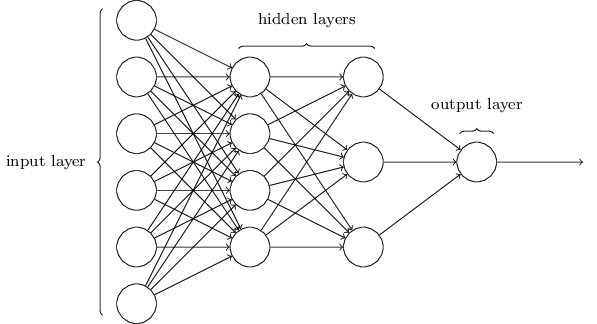
\includegraphics[scale=0.5]{./images/neural_net.png}
 \caption{{\it A common representation of a neural network: a single node works as the perceptron described above.}}
 \label{fig:ann}
\end{figure}

While the number of nodes in the input and output layers is fixed by the data under analysis, the best configuration of hidden layers is still an open problem.

The mathematical generalization from the perceptron is simple, indeed given the $i$-th layer its output vector $\bm{y}_i$ reads:  

\begin{equation}
 \bm{y}_i = \sigma(W_i \bm{y}_{i-1} + \bm{b}_i)
\end{equation}

where $W_i$ is the weights matrix of layer $i$ and $\bm{b}_i$ is the $i$-th bias vector, equivalent to $w_0$ in the perceptron case.
The output of the $i$-th layer becomes the input of the next one until the output layer yields the network's answer. 

As before, $\sigma$ is the activation function which can be different for every node, but it usually differs only from layer to layer. 
The choice of the best function for a given problem is still an open issue.

In a supervised environment, the model output is compared to the desired output ({\it truth}) by means of a cost function. 
An example of cost function is the sum of squared error : 

\begin{equation}
  C(W) = \frac{1}{N} \sum_{j=1}^{N} (y_j - t_j)^2
\end{equation}

where $N$ is the dimensionality of the output space. $C$ is considered as a function of the model's weights only since input data and true label $t$ are fixed.

{\bf overcome perceptron problems}

Those architectures are {\it universal approximators}, that means given an arbitrarly complex function, there is a fully connected neural network that can approximate it.

This type of network is called {\it feed forward} because the information flows linearly from the input to the output layer: however, it exists a class of models called {\it Recurrent} where this is not the case anymore and feedback loop are possible, but they are outside the scope of this work. 

\subsection*{Gradient Descent}

To minimize the loss function an update rule for the weights is needed. 
Given a cost funtion $C(w)$, the most simple one is the gradient descent:
\begin{equation}
 w \leftarrow w - \eta \nabla_w C
\end{equation}
The core idea is to modify the parameters by a small step in direction that minimize the error function. 
The lenght of the step is given by the {\it learning rate} $\eta$, which is a hyperparameter chosen by the user, while the direction of the step is given by $-\nabla_w C$, which point towards the steepest descent of the function landscape.

\begin{figure}[h]
 \centering
 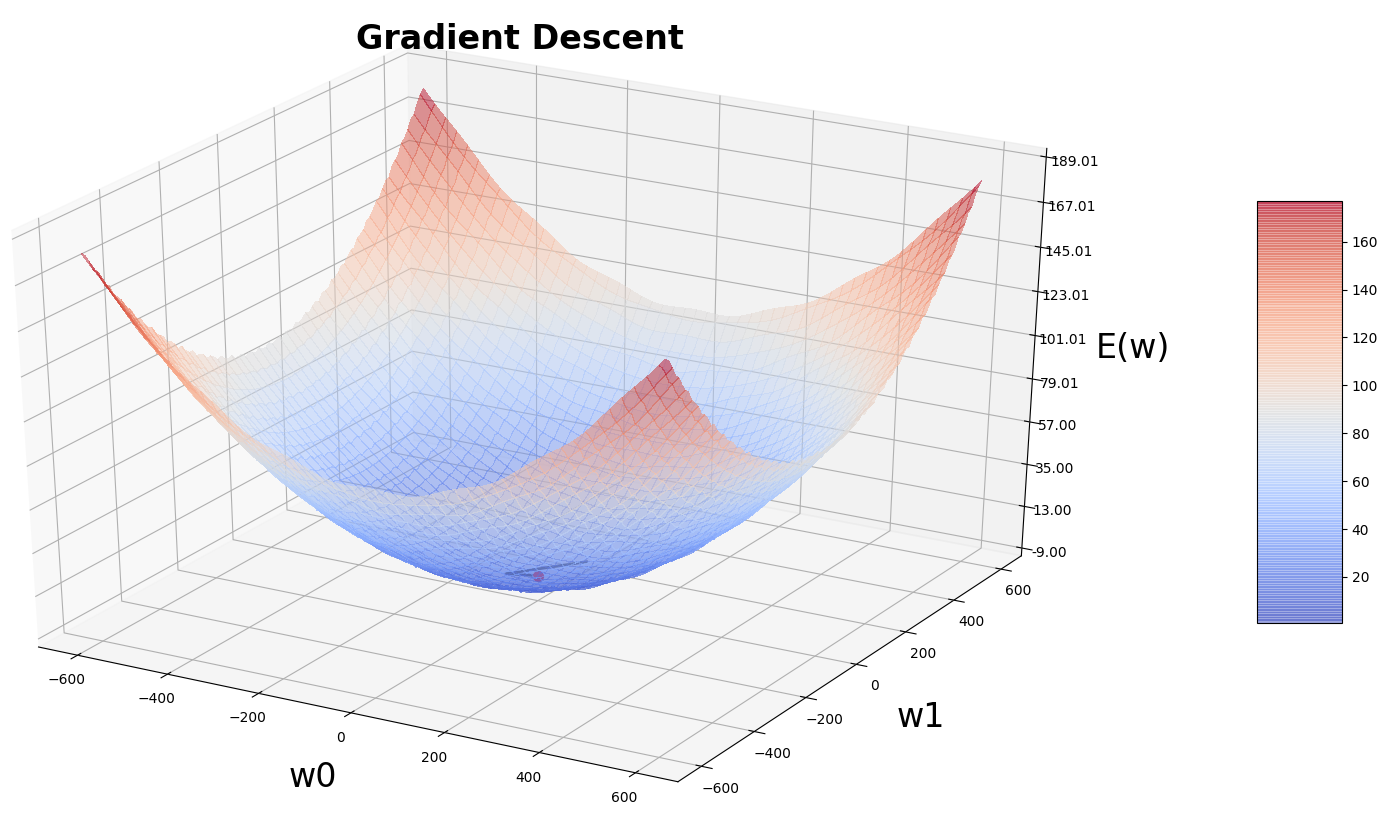
\includegraphics[scale=0.8]{./images/sgd.png}
 \label{fig:gd}
 \caption{\it Visual example of gradient descent for a model with 2 weights. The idea is to modify the weights to follow the direction of steepest descent for the landscape of the error function}
\end{figure}
The speed at which the algorithm converge to a solution and the precision of said solution are greatly influenced by the update rule. More complex and efficient update rules do exist, but they follow the same idea as the gradient descent.

\subsection*{Error Back Propagation}

The most common algorithm used to compute the updates to weights in the learning phase is the {\it Error Back Propagation}. 
Given a differentiable cost function $C(W)$, let's define :
\begin{align}
 \bm{z}_l &= W_l \bm{y}_{l-1} + \bm{b}_l  \\ 
 \bm{a}_l &= \sigma(\bm{z}_l)
\end{align}
respectively the de-activated and activated output vectors of layer $l$ for a model with $L$ total layer, and:
\begin{equation}
 \bm{\delta}_l = (\frac{\partial C}{\partial z_l^1}, \dots , \frac{\partial C}{\partial z_l^N}) 
\end{equation}
as the vector of errors of layer $l$. Then we can write the 4 equations of back propagation for the fully connected neural network \cite{neural-net-nielsen}:
\begin{align}
  &\bm{\delta}_L = \nabla_a C \odot \sigma'(\bm{z}_L) \\ 
  &\bm{\delta}_l = (W_{l+1}^T \bm{\delta}_{l+1}) \odot \sigma'(\bm{z}_l) \\
  &\frac{\partial C}{\partial b_l^j} = \delta_l^j \\
  &\frac{\partial C}{\partial w_l^{j k}} = a_{l-1}^k \delta_{l}^{j}
\end{align}
where  $\odot$ is the element-wise product.
Those equations can be generalized for others kind of layer, as I will show in the next chapters. 

The full training algorithm is : 

\begin{itemize}
 \setlength\itemsep{-0.3em}
 \item [-] define the model with random parameters
 \item [-] compute the output for one of the inputs
 \item [-] compute the loss function and the gradients
 \item [-] updates the parameters following the update rule, 
 \item [-] iterate from step 2 until the loss is sufficiently small
\end{itemize}

\section{Super Resolution}

The term Super-Resolution (SR) referes to a class of techniques which aim is to enhance the spatial resolution of an image, thus converting a given low resolution (LR) image to a corresponding high resolution (HR) one, with better visual quality and refined details.
Image super-resolution is also called by other names like image scaling, interpolation, upsampling and zooming \cite{survey-sr}.

There are many kind of super resolution {\bf FINISH}

\subsection*{Image Quality}

\subsection*{PSNR}
\subsection*{SSIM}

\section{Magnetic Resonance}


\chapter{Algorithms}

Brief Intro to the works on algorithm (NumPyNet, Byron, Layers, )

\section{Byron}

Byron (Build YouR Own Neural network) is a novel Deep Learning framework written in C++. 

\section{NumPyNet}

\section{Convolutional Neural Network}

A Convolutional Neural Network (CNN) is a specialized kind of neural network for processing data that has known grid-like topology \cite{Goodfellow-et-al-2016}. 
The name indicates that at least one of the functions employed by the network is a convolution. In a continuos domain the convolution between two functions $f$ and $g$ is defined as: 
\begin{equation}
 (f * g)(t) = \int_{-\infty}^{+\infty} f(\tau)g(t-\tau)d\tau
\end{equation}
The first function $f$ is usually referred to as the input and the second function $g$ as kernel. 
For Image Processing applications we can define a 2-dimensional discrete version of the convolution in a finite domain using an image $I$ as input and a 2 dimensional kernel $k$:
\begin{equation}
 C[i, j] = \sum_{u=-N}^N \sum_{v=-M}^M k[u, v] \cdot I[i-u, j-v]
\end{equation}
where $C[i, j]$ is the pixel value of the output image and $N$, $M$ are the kernel dimensions.
Practically speaking, a convolution is performed by sliding a kernel of dimension $N \times M$ over the image, each kernel position corresponds to a single output pixel, the value of which is calculated by multiplying together the kernel value and the underlaying pixel value for each cell of the kernel and summing all the results, as shown in figure \ref{fig:convolution}:

\begin{figure}[h]
 \centering
 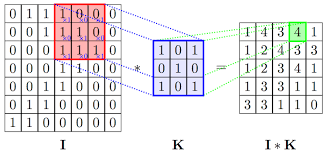
\includegraphics[scale=1.]{./images/conv.png}
 \label{fig:convolution}
 \caption{\it Visual example of convolution of an image I 7x7 with a 3x3 kernel K.}
\end{figure}

The convolution operation is also called $filtering$. By chosing the right kernel (filter) it is possible to highlight different features. For this reason the convolution operation is commonly used in image analysis: some of the most common applications are denoising, edge detection and edge enhancement. 

\section{Layers}

As described above, a neural network can be considered as a composition of function: for this reasons every Deep Learning library (e.g. Keras/Tensorflow, Pytorch, Darknet) implement each function as an independent object called {\it Layer}. 
By stacking different kinds of layer one after another, it is possible to build 

{\bf FINISH}

For the purposes of this work, I'm going to describe layers used in super resolution, however, Byron is developed also for different applications (object detection, classification, segmentation, style transfer, Recurrent NN etc...) and as such, many more layers are available.   

\subsection*{Convolutional Layer}

The convolutional layer object is the most used layer in DL Image Analysis, therefore its implementation must be  {\bf FINISH}

\subsection*{Pooling}
\subsection*{Shortcut Connections}
\subsection*{Pixel Shuffle}
\subsection*{Batch Normalization}
\subsection*{Loss Function}
\section{Timing}
\section{}

\chapter{Dataset and Methodology}

\section{Dataset}

\section{Models}

\chapter{Results}


\newpage
\nocite{*}
\bibliographystyle{abbrv}
\bibliography{biblio}

\end{document}
